\documentclass[12pt]{article}
\usepackage{amsmath,mathtools}
\usepackage[usenames,dvipsnames]{xcolor}
%\usepackage[bitstream-charter]{mathdesign}
\usepackage{microtype}
\usepackage[utf8]{inputenc}
\usepackage[T1]{fontenc}
\usepackage{libertine}
\usepackage[german]{babel}

%\usepackage{fontspec}
%\setmainfont{Corbel}
%\usepackage[libertine]{newtxmath}
\renewcommand{\familydefault}{\sfdefault}

\usepackage{graphicx}


\usepackage{siunitx}
\usepackage{fancyhdr}
\usepackage{sectsty}
\usepackage{setspace}
\usepackage{booktabs} % To thicken table lines
%\usepackage{chemstyle}
\usepackage[version=4]{mhchem}


\usepackage[ddmmyyyy]{datetime}
\renewcommand{\dateseparator}{.}

\pagestyle{fancy}

\cfoot{\thepage}

\lhead{Nevroz Arslan }
\rhead{\today}
\setlength{\headheight}{15pt}

\usepackage{overcite}
\renewcommand\citeform[1]{[#1]}

%\renewcommand*\printatom[1]{{\fontsize{10}{12}\selectfont\ensuremath{\mathsf{#1}}}}
\sectionfont{\fontsize{12}{15}\selectfont}

\makeatletter
    \setlength\@fptop{0\p@}
\makeatother


\newcommand\textbox[1]{%
  \parbox{.333\textwidth}{#1}%
}


\setlength{\headheight}{15pt}
 \sisetup{
        detect-all %,               %% Benutze gleiche Schriftarten wie im Text
    }
\renewcommand{\thesection}{\arabic{section}.}
\renewcommand{\thesubsection}{\thesection\arabic{subsection}}
\renewcommand{\headrulewidth}{0pt}
\begin{document}

\begin{onehalfspace}
  {\hfil  \textbf{\large Darstellung von Tetrakis(trimethylsilyl)silan}\hfil}
\par
  \vspace{1cm}
\hfil \textbf{Präparat Nr. 4 von 4 }\hfil
\section{Reaktionstyp: \textnormal{1. Salzmethatese 2. Metall-Halogen-Austausch}  }
\begin{figure}[!ht]
   \centering
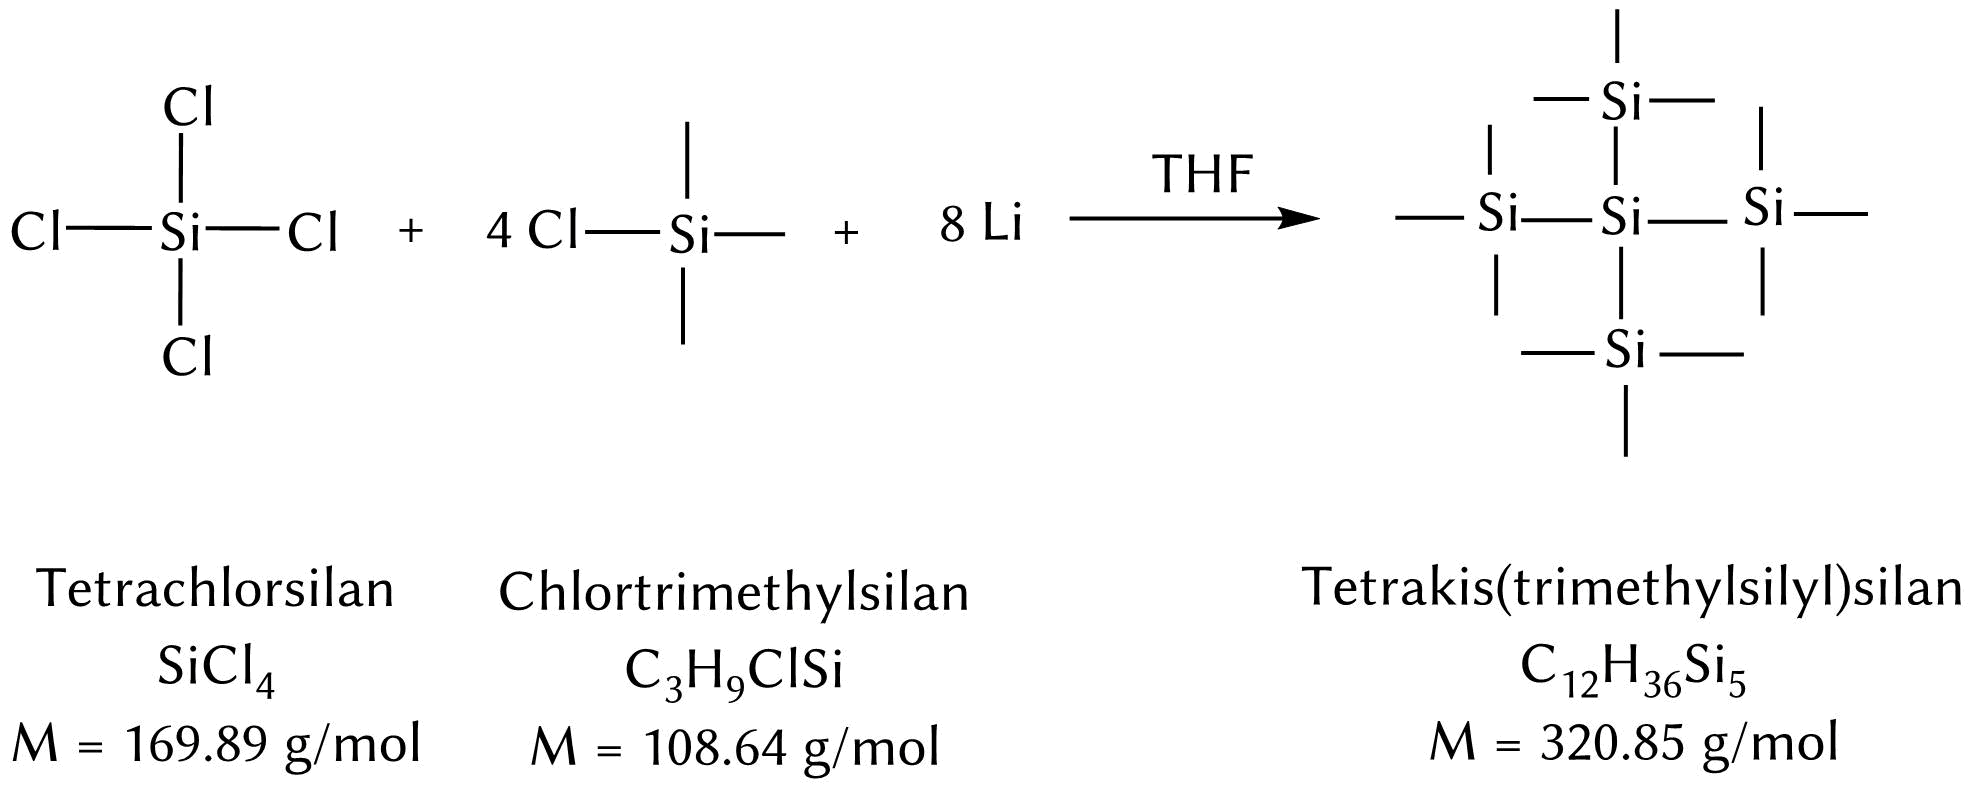
\includegraphics[width=\textwidth]{reaktion.png}
\end{figure}


\section{Berechnung des Ansatzes: }
Es sollten aus 7.00 g (1 \si{\mol}) \ce{Li} Tetrakis(trimethylsily)silan hergestellt werden.
Die Umrechnung des Literaturansatzes\cite{silicongilman} ergab folgenden Ansatz:\\\\
\noindent
\begin{tabular}{lrrrr}
\toprule
\textbf{ Bezeichnung }&\textbf{M [\si{\gram\per\mol}]} & \textbf{ n [\si{\mol}]} & \textbf{Menge} &  \textbf{Equiv}\\
Li             & 6.94    & 1.00 & 7.00 \si{\gram}          & 1.00 \\
Chlortrimethylsilan  & 108.64  & 0.40  & 51.2 \si{\milli\liter} & 0.40  \\
Tetrachlorsilan       & 169.89  &  0.08  & 9.2 \si{\milli\liter}  & 0.08 \\
THF            &         &      &         175 ml         &  LM  \\
\end{tabular}

 \section{Durchführung \cite{silicongilman}}
Zur Darstellung des Tetrakis(trimethylsily)silans wurde ein 500-ml-Dreihalskolben, der mit einem Rückflusskühler und Tropftrichter ausgestattet ist, ausgeheizt und mit Inertgas gespült. In dem Kolben wurde zuerst
 Tetrahydrofuran (100 \si{\milli\liter}) vorgelegt und danach Lithium (7.00 \si{\gram}, 1.00 \si{\mol}) hinzugegeben. Anschließend wurde unter Rühren  
 Chlortrimethylsilan (51.2 \si{\milli\liter}, 0.400 \si{\milli\mol}) hinzugetropft. Der Tropftrichter wurde mit Tetrachlorsilan (9.20 \si{\milli\liter}, 80 \si{\milli\mol}) in Tetrahydrofuran (75 \si{\milli\liter}) befüllt. Danach wurde ein Teil der Tetrachlorsilan-Tetrahydrofuran-Mischung (7.5 \si{\milli\liter}) zum Reaktionsmillieu zugetropft. Die Reaktionssuspension wird auf 70 \si{\celsius} erwärmt und unter Rühren für vier Stunden bei dieser Temperatur gehalten. Im Anschluss wurde zur Suspension im Laufe von vier Stunden die restliche Tetrachlorsilan-Tetrahydrofuran-Mischung kontinuerlich zugetropft und dann über Nacht bei Raumtemperatur gerührt. Zur Aufarbeitung wurden zunächst das Lithium und das ausgefallene Salz abfiltriert. Das Filtrat wurde mit einem Eis-Salzsäure-Gemisch (150 \si{\milli\liter}) hydrolysiert. Die organische Phase wurde abgetrennt, mit Tetrahydrofuran extrahiert, über \ce{MgSO_4} getrocknet und das Lösungsmittel wurde am Hochvakuum entfernt. Das Rohprodukt wurde danach aus Ethanol umkristallisiert. Die ausgefallenen Kristalle wurden mit Ethanol über Büchnertrichter gewaschen und das Lösungsmittel wurde am Hochvakuum entfernt. Das Produkt (11.44 g, 35.6 mmol, 45 \%) wurde als farbloser Feststoff erhalten.

\section{Ausbeute}
\begin{tabular}{ rl}
  25.66 g (80.0 mmol) =  & 100 \%\\
  11.44 g (35.6 mmol) =  & 45 \% (Lit.\cite{silicongilman} : 70 \%) \\
 \end{tabular}
\newpage
\section{Spektrenauswertung}
\begin{figure}[!ht]
   \centering
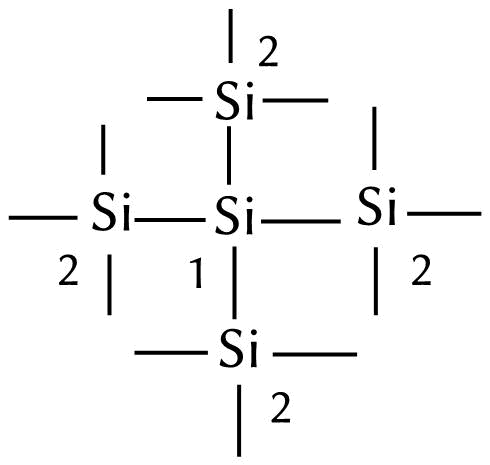
\includegraphics[scale=0.3]{auswert.png}
\end{figure}
\noindent
\textbf{\ce{^1_{}H-NMR}} (500 MHz, T = 305 \si{\kelvin}, \ce{CDCl_3}): \sffamily \ce{$\delta$} =
0.00 (s, 36 H, \ce{CH_3}). \\
\noindent
\textbf{\ce{^{29}_{}Si \{^1_{}H\}-NMR}} (100 MHz, T = 305 \si{\kelvin}, \ce{CDCl_3}): \sffamily \ce{$\delta$} =
- 9.8 (s, \ce{Si-CH_3}),
- 135.1 (s, \ce{Si}).


\section{Mechanismus\cite{silicongilman}}
In dem ersten Schritt der Reaktion findet eine Salz-Metathese statt. Dies wird durch einen Einelektronentransferschritt eingeleitet.
Das Lithium(0) (\textbf{2}) gibt ein Elektron ab und reduziert dabei das Tetrachlorsilan (\textbf{1}) unter Abspaltung des Chloridions.
Das gebildete intermediären Radikal (\textbf{3}) rekombiniert mit Lithium zum Lithiumtrichlorsilenid(II) (\textbf{4}). In dem nächsten Schritt der Reaktion 
erfolgt es ein Metall-Halogen-Austausch. Das nukleophile Trichlorsilylanion \textbf{4} addiert an das elektrophile Silicium des Chlortrimethylsilans (\textbf{5}) unter Abspaltung des Chlorids. Es entsteht dabei 1,1,1-Trichlor-2,2,2-Trimethyldisilan (\textbf{6}). Im Zuge der Bildung des Tetrakis(trimethylsily)silans (\textbf{7}) findet der oben beschriebene Reaktionsweg mehrmals statt. Die Trimethylsilylgruppe wird so lange addiert, bis die Chloride des 1,1,1-Trichlor-2,2,2-Trimethyldisilans (\textbf{6}) erschöpft sind. Die mehrmalige Substitution am 1,1,1-Trichlor-2,2,2-Trimethyldisilan (\textbf{6}) führt zum Produkt Tetrakis(trimethylsily)silan (\textbf{7}).\\
\begin{figure}[!htbp]
   \centering
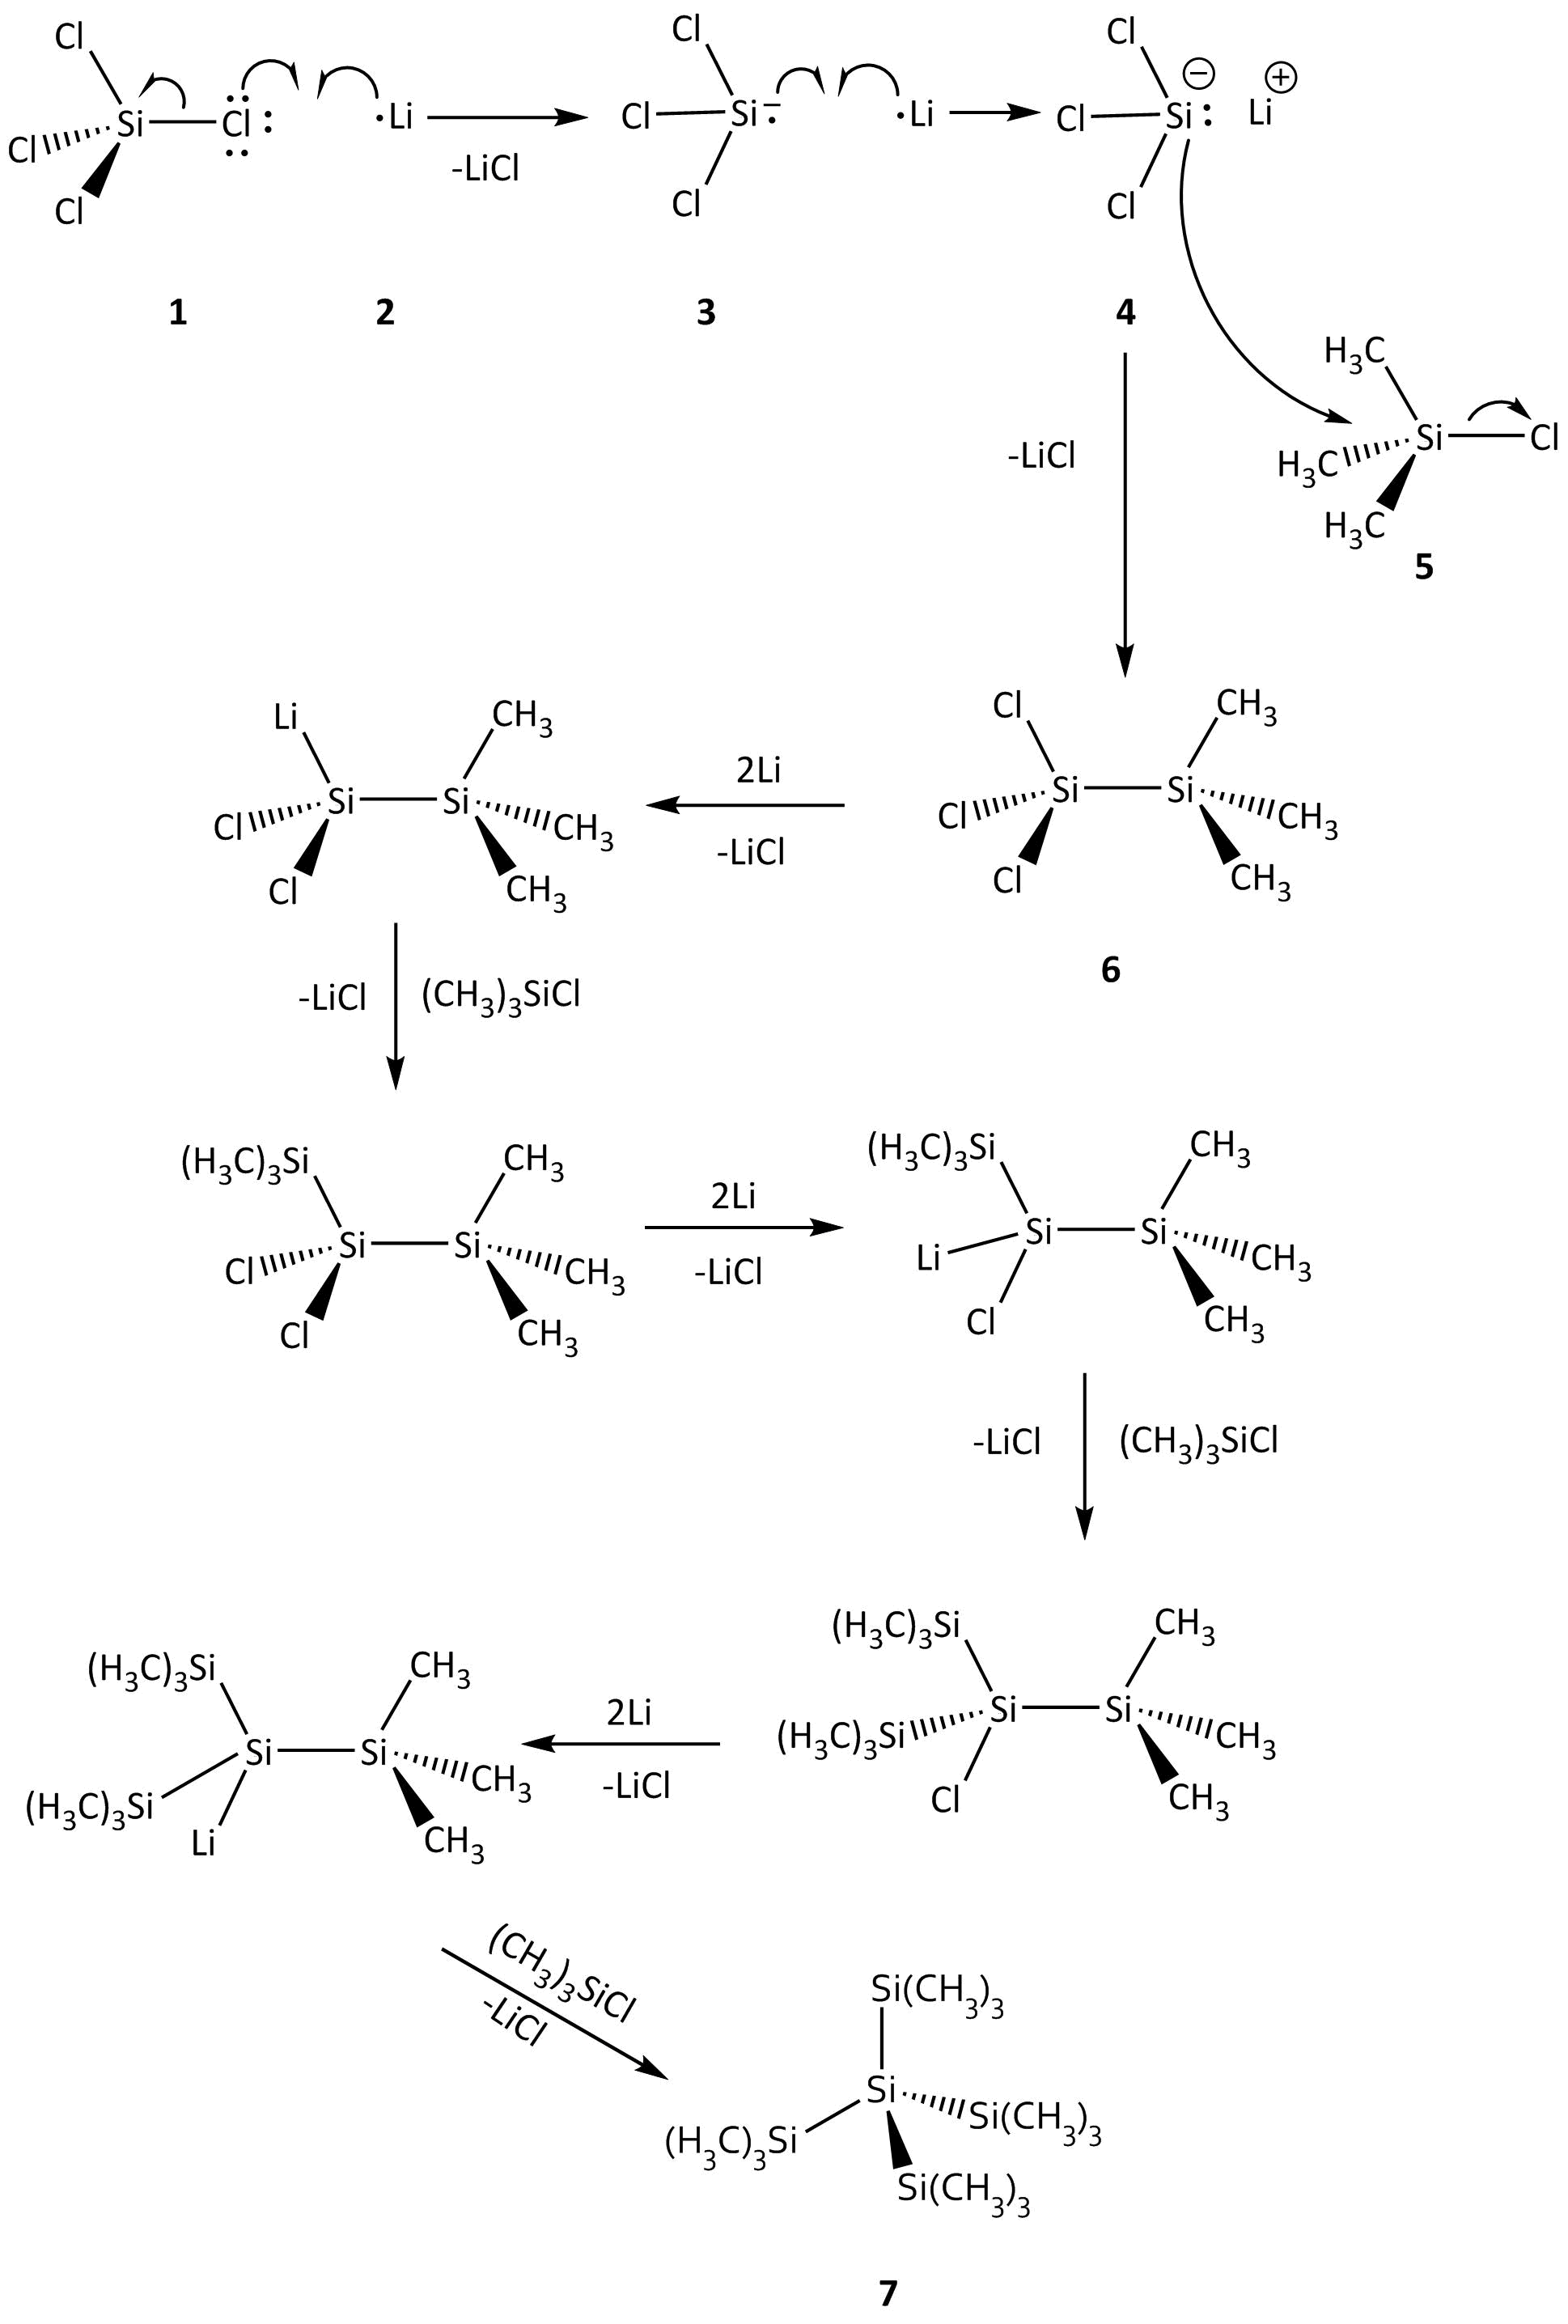
\includegraphics[scale=0.3]{mechan.png}
\end{figure}
\newpage

\section{Abfallentsorgung:}
Der Rest des Lithiums, das von der Reaktion übriggeblieben war, wurde mit Ethanol zerstört. 
Das im Rotationsverdampfer abgetrennte Lösungsmittel wurde im Behälter für halogenfreie Kohlenwasserstoffe entsorgt.
Die nach dem Hydrolysieren ausgefallenen Lithiumsalze wurden in den Feststoffbehälter gegeben.

\section{Literatur}
\renewcommand{\section}[2]{}%
\begin{thebibliography}{}
\bibitem{silicongilman}
H. Gilman, C. L. Smith, \textit{J. Organometal. Chem.} \textbf{1967}, 245 - 253.
\end{thebibliography}
\end{onehalfspace}
\end{document}